\chapter{A játék működése}

\thispagestyle{fancy}
\pagestyle{fancy}
\section{Játék ismertetése}
A játék melyet lefeljleszettem, a közismert memória játék. A játékot lehet egyedül, vagy akár többen is játszani.

A játékban, egy asztalon 6, 8, 10 vagy 12 pár kártya található, képpel lefelé fordítva ahogyan az a \ref{img:asztal}. ábrán is látható.
A kártyák előlapján betűk találhatók. Egyjátékos esetben a játékos célja, hogy minél kevesebb kártyapár megfordításából megtalálja az összes memória párt. Többjátékos esetben, hogy ő szerezze a legtöbb pontot, vagyis több kártyapárt fordítson fel, mint az ellenfelei.

Ahhoz, hogy egy kártyát megfordítson, a játékosnak rá kell kattintania. Ekkor láthatóvá válik, mely betűhöz tartozik a memória elemhez (\ref{img:kartya_fliped}. ábra). 
A megfordított kártyához választani kell egy másikat. A játékosnak törekednie kell, hogy korábbi ismeretei alapján, hogy a következőre a választott kártya előlapján ugyanaz a betű szerepeljen, mint a már felfordított memória lapon, vagyis egy párt fordítson fel. 
Értelemszerűen ez az első felfordításkor nem lehetséges, hiszen nincs korábbi ismerete a játékról (\ref{img:non_pair}. ábra).

Ha a felfordított kártyák nem alkotnak párt, akkor a kártyák maguktól visszafordulnak pár másodperc elteltével. Ez után egyszemélyes játék esetén esetén végrehajtunk egy újabb fordítást. Többjátékos esetén a következő játékos végezheti el a körét. 

Ha párt alkotnak, akkor a kártyákat magunkhoz vehetjük. Ez mutatja a pontunkat, mely csak többjátékos esetben fog számítani.




\begin{figure}
    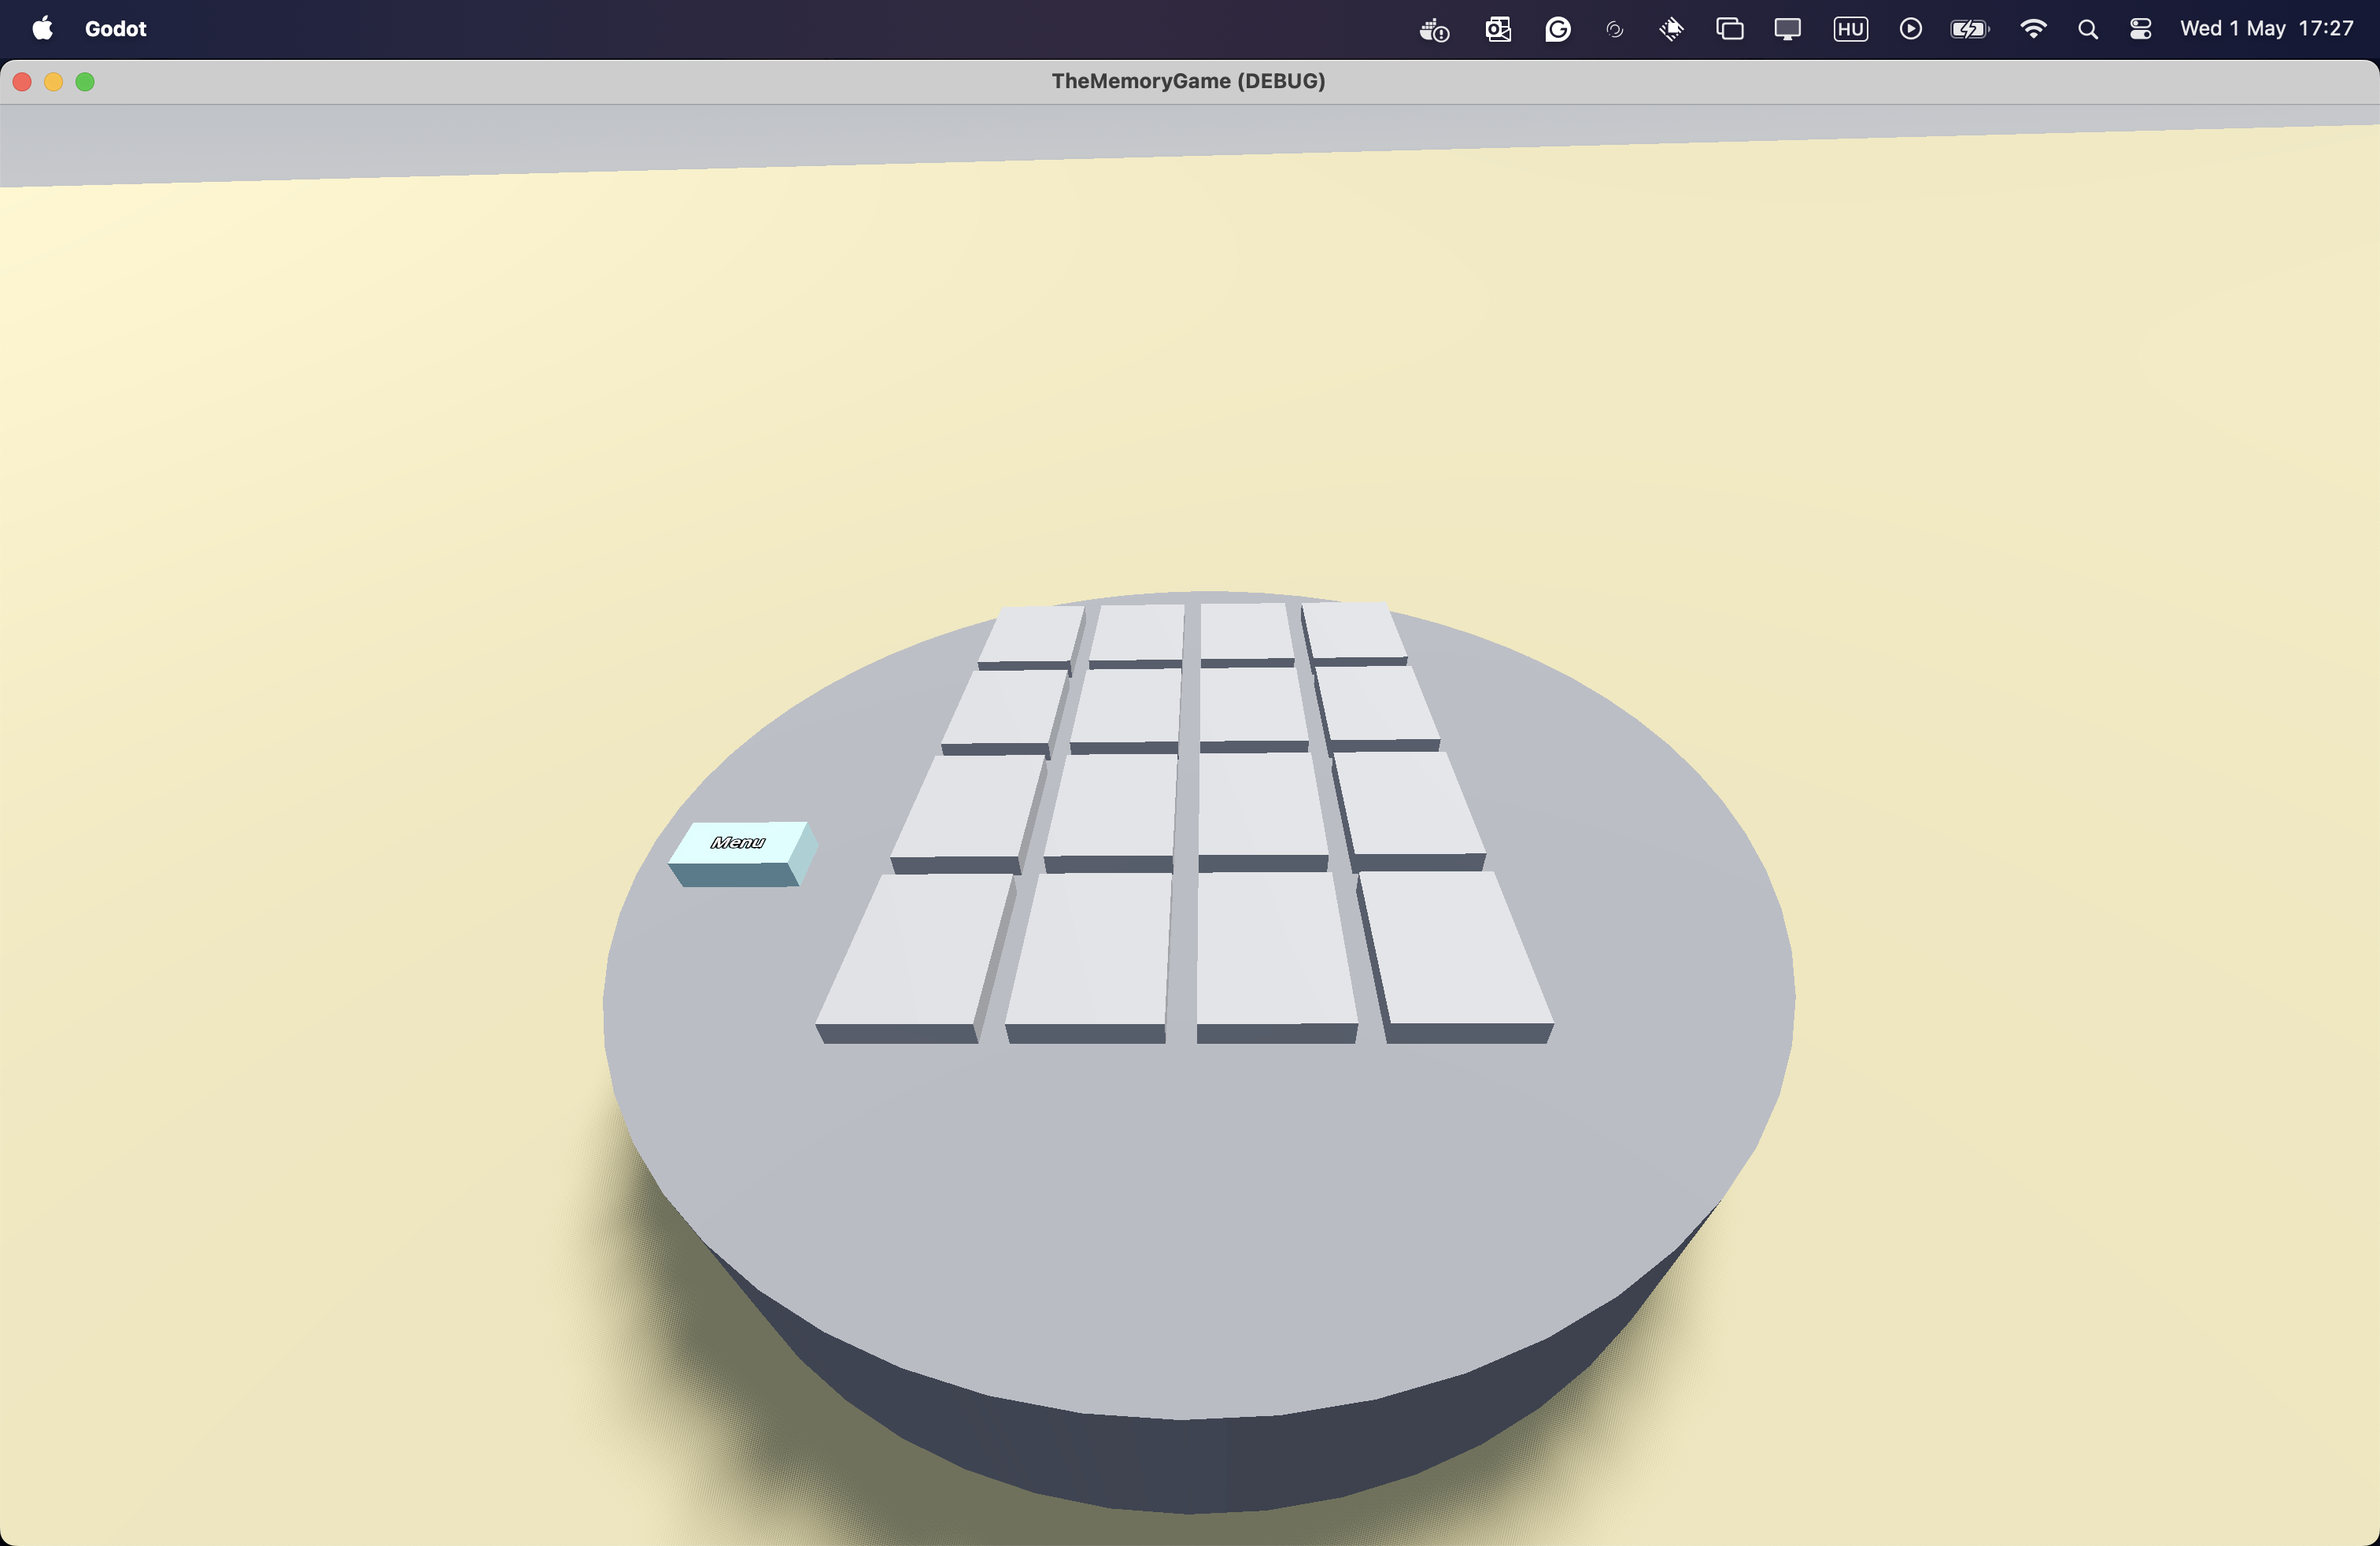
\includegraphics[width=\textwidth]{img/asztal_4x4.png}
    \caption{4x4-es memóriajáték kezdő állapota}
    \label{img:asztal}
\end{figure}
\begin{figure}
    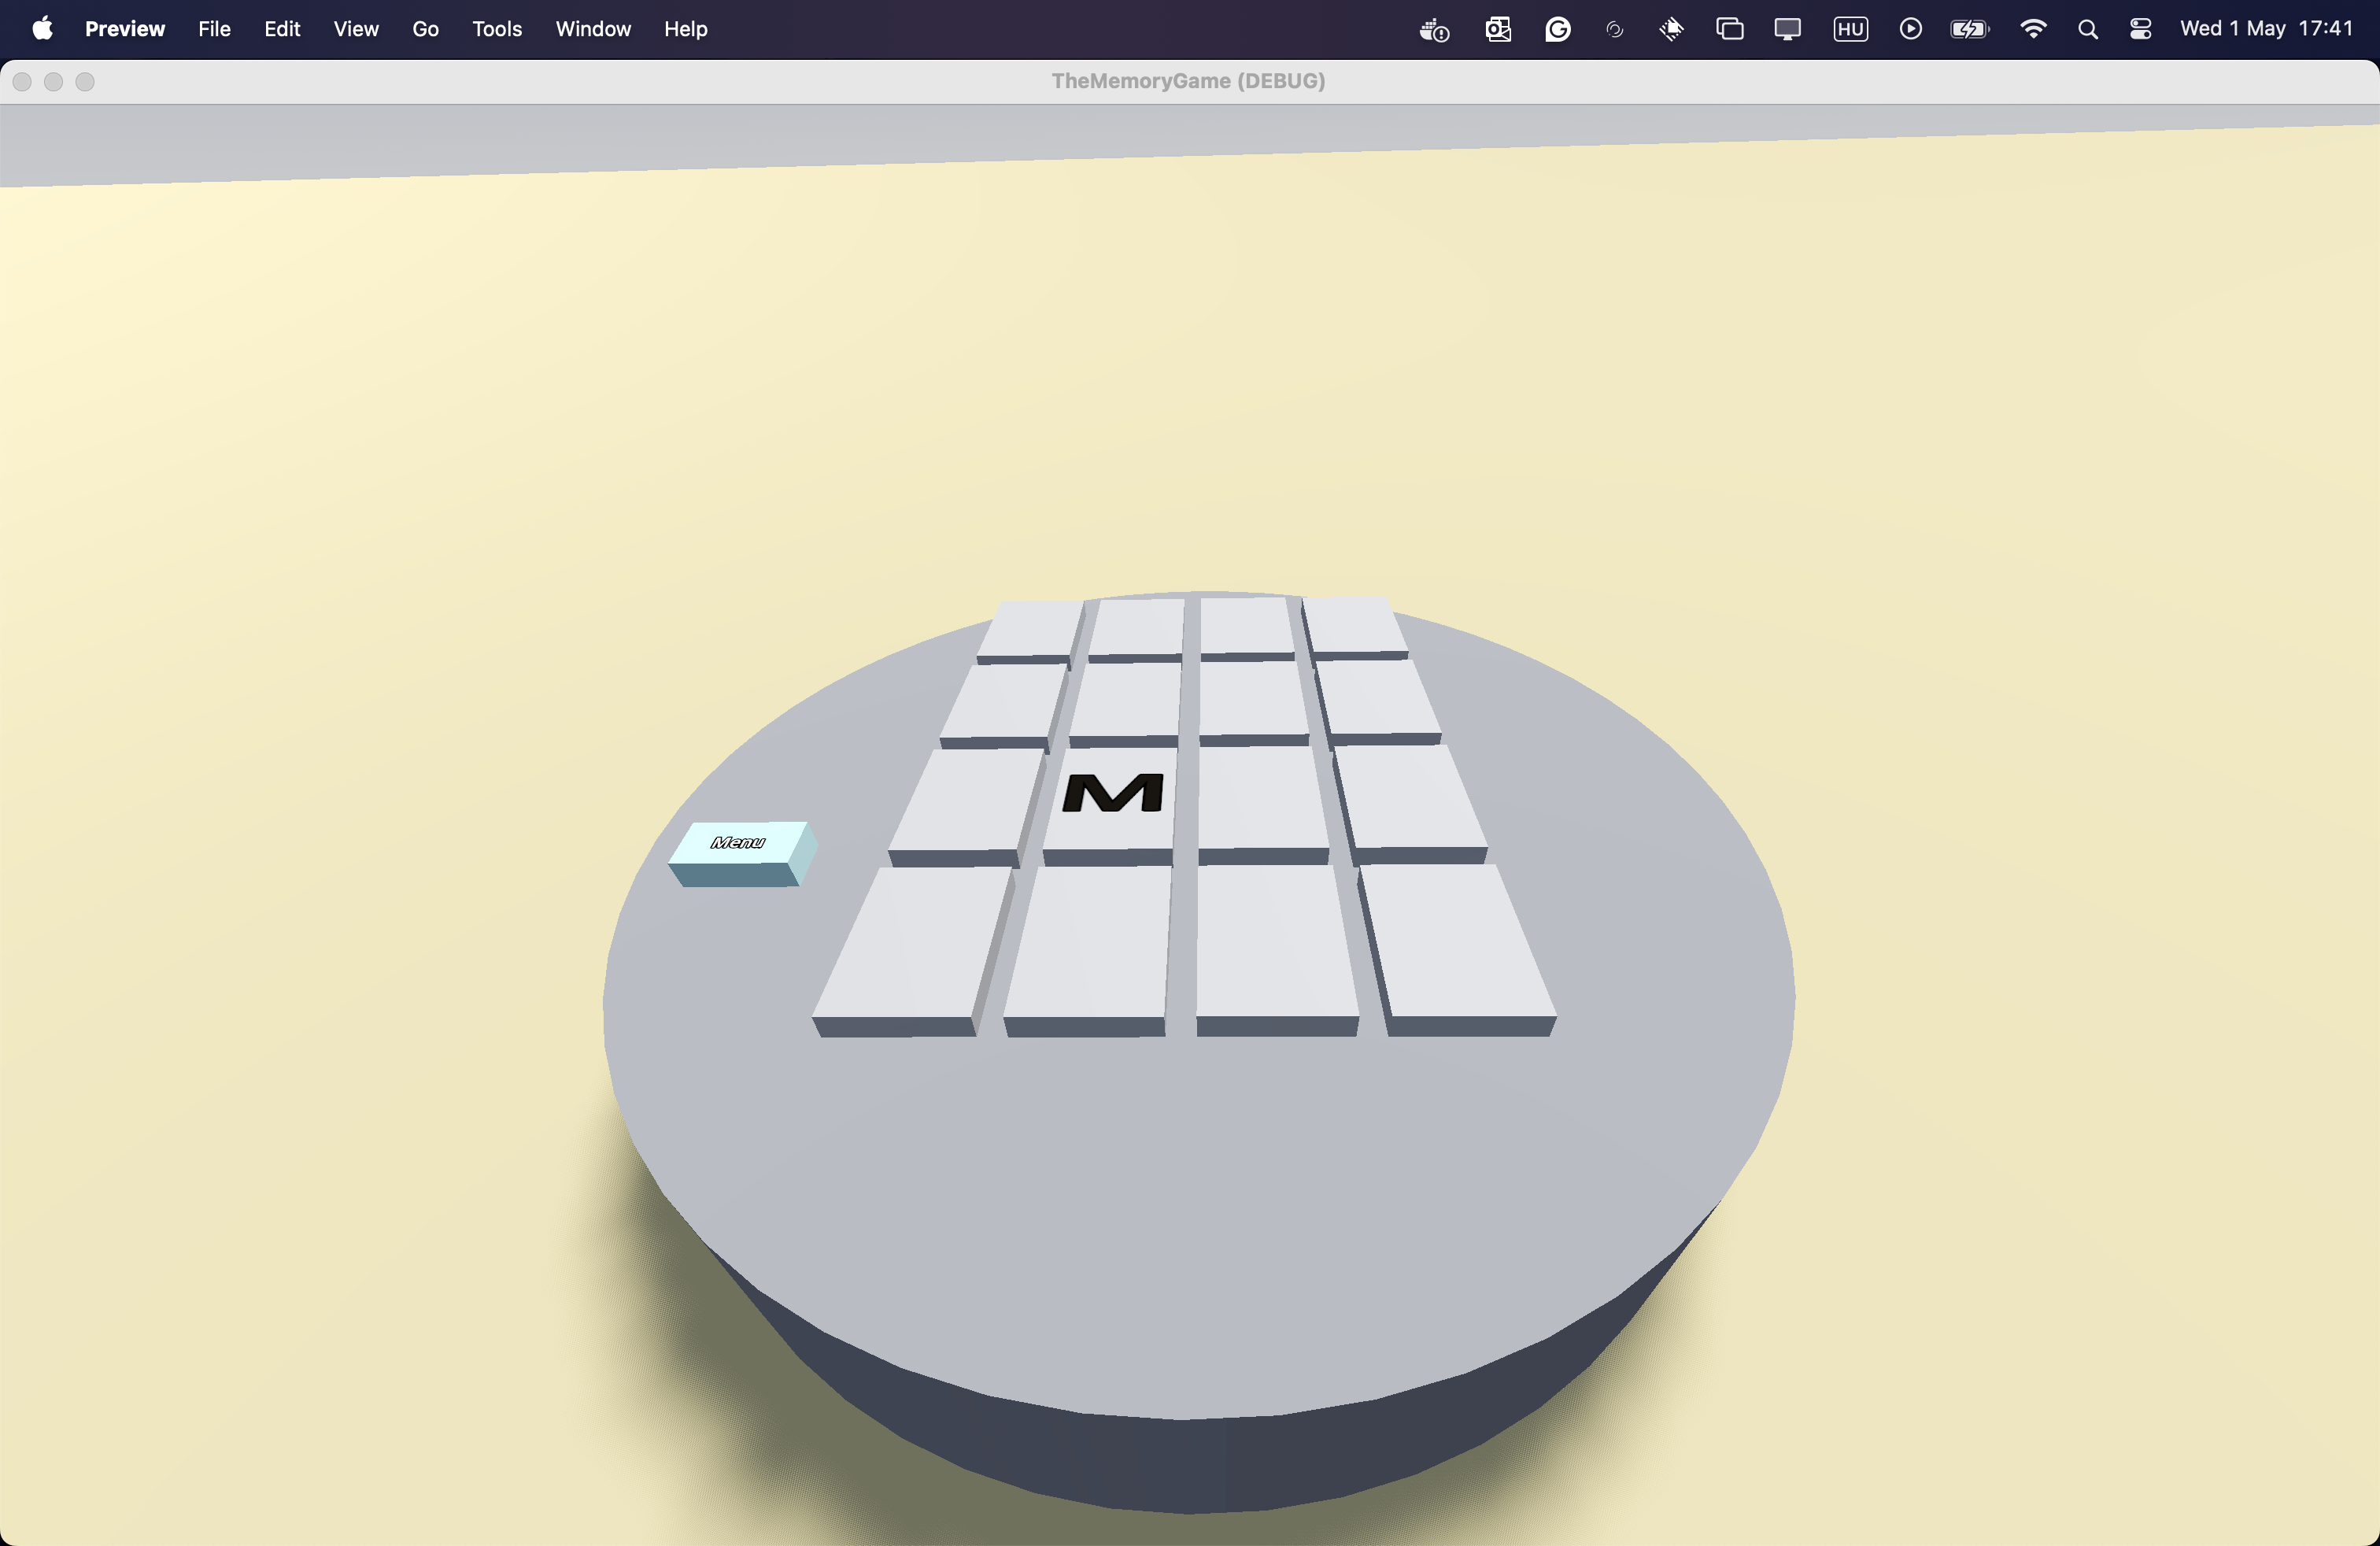
\includegraphics[width=\textwidth]{img/asztal_4x4_card_flipped.png}
    \caption{4x4-es memóriajáték egy kártya ki van választva}
    \label{img:kartya_fliped}
\end{figure}
\begin{figure}
    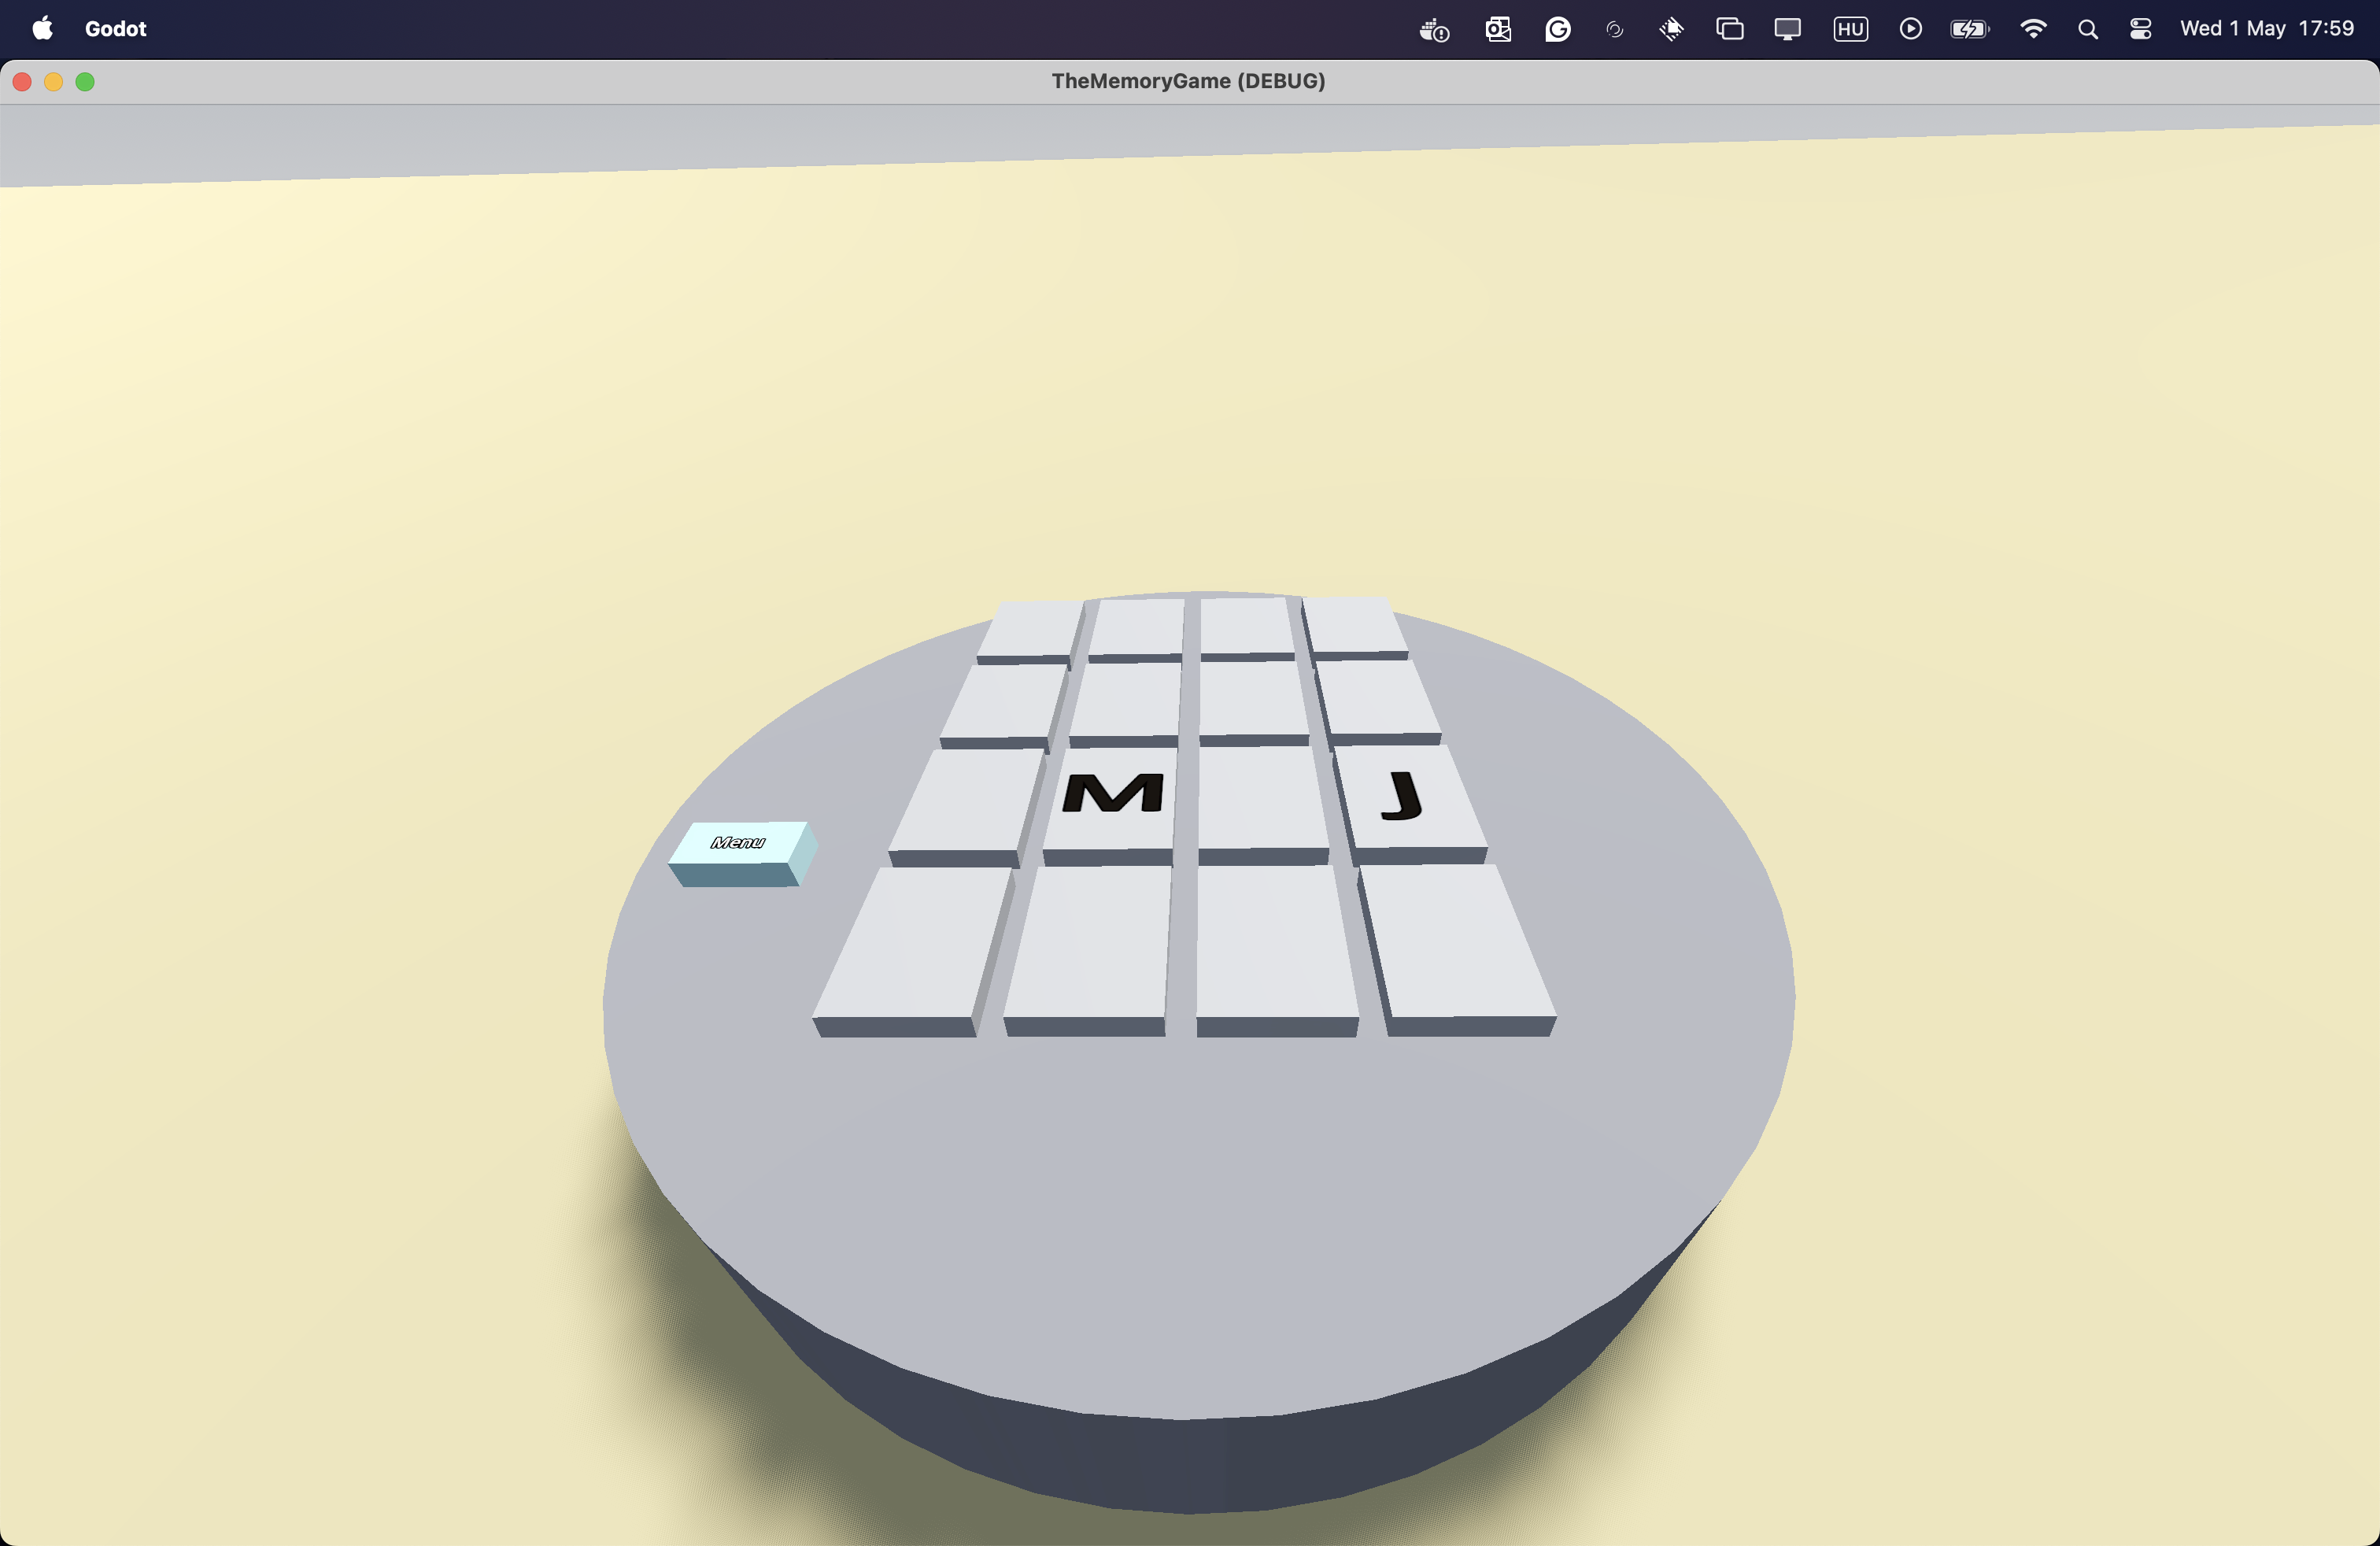
\includegraphics[width=\textwidth]{img/asztal_4x4_non_pair.png}
    \caption{4x4-es memóriajáték. Mivel a betűk nem azonosak, ezér ez nem egy pár, visszafordítjuk a kártyákat.}
    \label{img:non_pair}
\end{figure}